%%
%% This is file `sample-sigconf.tex',
%% generated with the docstrip utility.
%%
%% The original source files were:
%%
%% samples.dtx  (with options: `sigconf')
%% 
%% IMPORTANT NOTICE:
%% 
%% For the copyright see the source file.
%% 
%% Any modified versions of this file must be renamed
%% with new filenames distinct from sample-sigconf.tex.
%% 
%% For distribution of the original source see the terms
%% for copying and modification in the file samples.dtx.
%% 
%% This generated file may be distributed as long as the
%% original source files, as listed above, are part of the
%% same distribution. (The sources need not necessarily be
%% in the same archive or directory.)
%%
%%
%% Commands for TeXCount
%TC:macro \cite [option:text,text]
%TC:macro \citep [option:text,text]
%TC:macro \citet [option:text,text]
%TC:envir table 0 1
%TC:envir table* 0 1
%TC:envir tabular [ignore] word
%TC:envir displaymath 0 word
%TC:envir math 0 word
%TC:envir comment 0 0
%%
%%
%% The first command in your LaTeX source must be the \documentclass command.
\documentclass[sigconf]{acmart}

\usepackage{listings}
\usepackage{graphicx}
\usepackage{graphics}
\usepackage{geometry}
\usepackage{xcolor}
\usepackage{anyfontsize}

\definecolor{codegreen}{rgb}{0,0.6,0}
\definecolor{codegray}{rgb}{0.5,0.5,0.5}
\definecolor{codepurple}{rgb}{0.58,0,0.82}
\definecolor{backcolour}{rgb}{0.95,0.95,0.92}
\lstdefinestyle{mystyle}{
    backgroundcolor=\color{backcolour},
    commentstyle=\color{codegreen},
    keywordstyle=\color{magenta},
    numberstyle=\color{codegray},
    stringstyle=\color{codepurple},
    basicstyle=\ttfamily\footnotesize,
    breakatwhitespace=false,
    breaklines=true,
    captionpos=b,
    keepspaces=true,
    numbers=left,
    numbersep=5pt,
    showspaces=false,
    showstringspaces=false,
    showtabs=false,
    tabsize=2
}
\lstset{style=mystyle}

%% Rights management information.  This information is sent to you
%% when you complete the rights form.  These commands have SAMPLE
%% values in them; it is your responsibility as an author to replace
%% the commands and values with those provided to you when you
%% complete the rights form.
\setcopyright{acmcopyright}
\copyrightyear{2023}
\acmYear{2023}
\acmDOI{XXXXXXX.XXXXXXX}

%% These commands are for a PROCEEDINGS abstract or paper.
\acmConference[ICCDA '23]{}{July, 2023}{GuiYang, CN}
\acmPrice{15.00}
\acmISBN{978-1-4503-XXXX-X/23/07}

%%
%% Submission ID.
%% Use this when submitting an article to a sponsored event. You'll
%% receive a unique submission ID from the organizers
%% of the event, and this ID should be used as the parameter to this command.
%%\acmSubmissionID{123-A56-BU3}

%%
%% For managing citations, it is recommended to use bibliography
%% files in BibTeX format.
%%
%% You can then either use BibTeX with the ACM-Reference-Format style,
%% or BibLaTeX with the acmnumeric or acmauthoryear sytles, that include
%% support for advanced citation of software artefact from the
%% biblatex-software package, also separately available on CTAN.
%%
%% Look at the sample-*-biblatex.tex files for templates showcasing
%% the biblatex styles.
%%

%%
%% The majority of ACM publications use numbered citations and
%% references.  The command \citestyle{authoryear} switches to the
%% "author year" style.
%%
%% If you are preparing content for an event
%% sponsored by ACM SIGGRAPH, you must use the "author year" style of
%% citations and references.
%% Uncommenting
%% the next command will enable that style.
%%\citestyle{acmauthoryear}

%%
%% end of the preamble, start of the body of the document source.
\begin{document}

%%
%% The "title" command has an optional parameter,
%% allowing the author to define a "short title" to be used in page headers.
\title{Projit: An Open Source tool for Decoupled Data Science}

%%
%% The "author" command and its associated commands are used to define
%% the authors and their affiliations.
%% Of note is the shared affiliation of the first two authors, and the
%% "authornote" and "authornotemark" commands
%% used to denote shared contribution to the research.
\author{John Hawkins}
\email{john.hawkins@Getting-Data-Science-Done.com}
\orcid{1234-5678-9012}
\affiliation{%
  \institution{Getting-Data-Science-Done.com}
  \city{Sydney}
  \state{NSW}
  \country{Australia}
  \postcode{2000}
}

\renewcommand{\shortauthors}{Hawkins}

\begin{abstract} 
Scientific practice has expanded to become increasingly dependent of digitial technologies,
large scale data processing and analytical methods for working with large data volumes. 
These shifts have demanded new methods of implementing and recording the details of 
scientific projects. Monolothic applications have the advantage of a single and 
consistent design, however they impede the ability of users to innovate and 
incrementally improve processes. We discuss the qualities of an ideal eScience 
framework for building multi-stage collaboration scientific workflows and present 
an open source implementation for managing scientific processes in a decoupled 
fashion that permits both flexible implementation of any stage of processing, 
and greater ease of meta-data analysis.
\end{abstract}


\keywords{Data Science, Experiment Tracking, Reproducible Science, Metadata Tracking}

\maketitle

\section{Introduction}

Progress in scientific research depends heavily on accurate record keeping of previous
experimental approaches and results. Failure to maintain these records impedes progress
by making it difficult to reproduce work, or imposing the costs of repeatedly testing 
failed lines of experimentation. This cost becomes particularly high in the age of the
reproducibility crisis where many teams are running the same experiments in parallel, without
knowledge of each others work, and producing a factory line of un-reproducible results 
\cite{Ioannidis2005}. This cost is compounded by the problems of increasingly 'Big Data' 
based science, where the logistics of maintaining and tracking data sets is challenging.
While big data may offer many opportunities cross-disciplinary and algorithmic science\cite{Schmitt2015}, 
there is a strong concern that this will be limited\cite{Succi2019}, 
and that the core scientific tasks of conceiving,
designing and running experiments needs to be managed at an ever increasing scale.

Software approaches to managing scientific data, processes and meta-data are typically referred to 
as e-science platforms. In general they are either built as front-ends for specific 
scientific domains \cite{Howe2008,Pettit:2010} (leveraging known analytical practices in
the given domain) or they are designed to faciliate interoperability between different
technology stacks \cite{Subramanian2013}. Machine learning focused frameworks tend to 
focus on solving problems of model training and deployment for specific technologies\cite{Alberti:2018,MolnerDomenech:2020}, and hence have limited generality.

Platforms for eScience offer a variety of solutions for these problems including  
tracking the lineage and management of data, referred to as 
the provenance problem \cite{Sahoo:2008,Conquest:2021}.
The goal of provenance frameworks is sufficient auditibiliy of data that will 
render eScience transparent and repeatable. This can be auditing of data from multiple 
source systems, or auditing of logs generated during data processing\cite{Ferdous2020}. 
At the extreme we can seek to quantify every transformation that happens to data in 
the course of processing\cite{Sahoo2009}. Regardless of the
specific data to be audited, these frameworks focus on developing unified systems and 
processes so that auditing can be easily performed over many projects. It has been 
argued that tracking meta-data is critical for the endeavour of large scale open and auditable 
science\cite{Reznik2022}. It is only through meta-data that we are able to build frameworks
that can understand and assist the scientific process.

In addition to systems for tracking data, eScience application may include facilities
for orchestration of data processes and external services\cite{Subramanian2013}, 
requests for experiments with specific parameters\cite{Hunter:2005}, 
or integrated analysis of results, generation of insights and documentation. 
Other frameworks and approaches in eScience focus on understanding how to do large 
scale collaborative science, or facilitate meta-level learning of various 
kinds\cite{Hunter:2005,Liu:2023}. The better we track the
process of science as a whole, the better we can understand both how to improve 
scientific processes as well as data mine the history of experimental results for 
phenomena that are difficult to detect.

Frameworks for eScience will typically need to take a position on the extent to which 
they are domain specific versus general purpose. A domain specific approach can 
integrate multiple data sources in a domain aware fashion that can faciliate 
automated or assisted scientific discovery\cite{Howe2008,Pettit:2010}. On the
other hand a general purpose framework facilitates multi-disciplinary collaboration 
and permits meta-analysis that transcends the boundaries of disciplines. 
The other key dimension for a decision is the extent to which an eScience 
application depends on specific technologies, many machine learning science platforms
can provide efficiency gains, but only when using specfic libraries and 
frameworks\cite{Alberti:2018,MolnerDomenech:2020}. Similarly, other empirical 
science platforms are built on specific database, webservers or application
frameworks, which make them less extensible and harder to integrate.

Many Machine Learning experimentation frameworks focus on the task of making experiments
easier to execute and deploy into production systems\cite{Alberti:2018,MolnerDomenech:2020}.
To do so they are often constructed for specific combinations of technology.
This is often necessary limitation to either make a project feasible or enable efficiency,
but it has the side-effect of limiting general applicability. An ideal data science
framework would allow open ended experimentation, with an ability for easy tracking
and comparison of these experiments.

\begin{figure*}
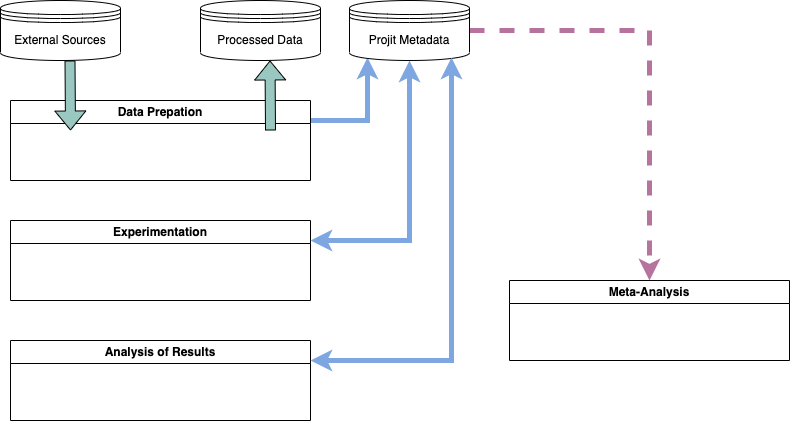
\includegraphics[scale=0.6]{./images/Projit_decoupled_process.drawio.png}
\caption{Projit Process for Decoupled Data Science}
\label{fig:projit}
\end{figure*}

In this work we argue for the development of data science frameworks that impose minimal 
requirements, both in terms of appplication domains and underlying technologies. 
We present a design framework for building decoupled data science tools that can 
improve efficiency and replication through standardisation, without
unreasonable impositions on design decisions. We describe the design of a open 
source meta-data tracking project integration tool (\textit{projit}) that can be used either as a 
Command Line Application (CLI) or python API. Internally \textit{projit} depends 
only on a simple metadata store that uses the general purpose JSON format. 
As such it is trivial for developers to build interfaces in other
languages, or devise web service APIs for decentralised versions. We explore a 
case study for analysing a project for which we have used 
the \textit{projit} application to manage our experiment metadata.


\section{Methodology}

We begin by discussing the desirable features of an open science framework. 
These are drawn from observations of both how collaborative science works and the 
successful components of distributed scientific endeavours. These requirements are 
drawn from both sciences that are typically dependent on computational frameworks 
(computer science, bioinformatics, physics) and those that generally are not
(social science, psychology).

The key elements are as follows:

\begin{itemize}
 \item Sources: Provenance of Data Sources
 \item Processing: Records of Data Processing / Transformations
 \item Reuse: Tooling to Facilitate Reuse of Datasets
 \item Tracking: Tracking of Experiments and Outputs
 \item Results: Comparison of Methods and Results
 \item Documentation: Generation of Project Documentation
 \item Reproducibility: Facilitation of reproduction of results
 \item Meta-Analysis: Facilitation of Multi-Project Meta-Analysis
\end{itemize}

The elements in this list are organised in an approximately sequential manner. 
However, as we discuss them below it should be apparent that there are many ways 
in which these elements support each other.

First and foremost, data driven projects require access to the required \textbf{source} data 
and need to maintain records of the data provenance for \textbf{reproducibility}. 
There will typically be \textbf{processing} applied to these datasets to 
render them applicable to experimentation and analysis. An ideal tool will track the 
sequential nature of this \textbf{processing} as well as store information about 
the location of each resulting dataset. The data processed in this way is then 
available for \textbf{reuse} across experiments and analysis,
making \textbf{results} comparable.

The centralised storage of data in a unified format allows for scripted generation 
of \textbf{documentation}, and facilitates easy \textbf{meta-analysis}. If the 
product metadata is stored in a public or open source repository then it is 
possible to build tools that extract and process the data from multiple projects. It
will permit the emgergence of an ecosystem of tools that mine the history of 
experiments conducted on the same or similar source data, evaluate experimental 
protocols or algorithms across projects and potentially
automate some forms of \textbf{meta-analysis}.
 
To achieve these advantages we require a uniform system for storing all necessary 
data that are inputs and outputs for each stage of a data science experiment. 
The central store permits decoupling of processes by allowing each
element of the process to be implemented and executed independently of the others.

\subsection{Projit Process}

The central design principle of \textit{projit} is that the decoupling of data science 
should be achieved through utilisation of a simple metadata store. Each aspect of 
data science work can be allowed to proceed without awareness of the structure of 
any other element as long as it can access the information it requires through this
metadata store.

In Figure \ref{fig:projit} we see that the core steps of data preparation, experimentation
and analysis of results all happen independently. Each of them accesses the projit metadata 
store for the information they need, and subsequently store information and results once 
complete. This process means that in principle the location of an underlying dataset 
could change without modifying other elements of the project. Similarly, we might change 
the parameters or an experiment or the set of metrics we calculate. Each experiment and 
analysis task operates independently of the others, relying on the meta-data store for 
dependencies rather than direct communication. When changes are made there might be a
loss of synchronisation between elements, for example between test data and results. 
This issue can only be addressed by extending the project with a dependency graph for 
capturing, and potentially orchestrating, processing pipelines.

In addition to the dominant requirements of experimentation (parameters and results) we 
store the results of each experimental execution as well as the experiment duration, 
measured from the time of initiation to completion. These records are particularly 
important in data science and machine learning where we may want to trade off 
performance with computational requirements. But these values could be used to store
information about real world experimental execution or the time required to marshall 
and sequence a series of independent web services. 

The project utilises a notion of key asset types: dataset, experiment and results. Each
of these can be created independently with a reference between them in a loose coupling.
In addition, a tagging system allows these assets to be labelled with an open ended number
of tags that cen be used when extracting or tabulating project properties.

\subsection{Implementation}

Projit has been implemented as python package that functions as both a command line 
application and library that can be included inside other scripts and applications. 
The command line application can be used to query the project metadata in much the 
same way that the git application can be used to manipulate a query a set of software
source files. A user can add, modify and list the collection of assets in the 
project: datasets, experiments and results are all accessible from the command line 
application.

\begin{lstlisting}[language=BASH,label={code:install}, caption=Installation and Invocation of Projit CLI]
pip install projit

projit init "Test Project"
\end{lstlisting}

The python package can be included in a script so that the script can access the 
project metadata store. This allows the script to find the location of common 
datasets, register themselves as an experiment or execution and store results once 
the script is complete. Programmatic interaction with the project data through
the projit API is what permits the scripts of a project to be decoupled and 
contribute to the project without being aware of how any other element is 
structured or implemented. Furthermore, as the metadata
is stored locally in standard JSON files, these can be stored inside a cloud 
repository and then contributed to by collaborators. 
This allows distributed data science teams to define their own lines of experimentation,
but use a synchronised data set then continually contribute to a central meta-data 
store of project results.

\begin{lstlisting}[language=Python,label={code:usage}, caption=Usage of Projit Python Library]
import projit as pit

experiment_name = "My Experiment"
project = pit.projit_load()
exec_id = project.start_experiment(experiment_name, sys.argv[0], params={})
#
# EXPERIMENT EXECUTION CODE 
#
project.end_experiment(experiment_name, exec_id)
\end{lstlisting}


\section{Case Study}

We have utilised the projit application across multiple data science projects to store 
references to reusable datasets and experimental resultss. Additionally, the metadata store 
contains information about the number of times each experiment has been executed, 
and the execution time utilised on each run. This allows us to conduct an after-the-fact
investigation into these projects. In this section we demonstrate how some details of these
projects can be revealed through the project meta-data.

\subsection{Systematic Review with Machine Learning}

In a recent paper we explored the use of machine learning algorithms for filtering a initial
set of article abstracts as part of a systematic review\cite{HawkinsTivey2023}. 
The resulting paper focused on four
different machine learning strategies, the first of which were standard machine learning techniques
trained on simple features, such as the age of the article, the number of authors, the number of 
matching keywords in the abstract etc. The presentation of results in this paper created the impression
that all of these baseline models were executed in the first round of experimentation. By querying
the \emph{projit} meta-data store to fine the first execution time of each experiment, we created
Table \ref{tab:execs}, which shows that he Naive Bayes and SVM models were in fact executed last. 

\begin{table}
\caption{Experiment Executions}
\label{tab:execs}
\resizebox{\columnwidth}{!}{%
\begin{tabular}{|l|r|r|}
\toprule
Experiment            &Execution Count    &First Execution     \\
\midrule
Dataset Size         &1                   &2   \\
Variables            &11                  &1      \\
Outlier Proportion   &2                   &0  \\
Std Multiplier       &6                   &     \\
\bottomrule
\end{tabular}
}
\end{table}

In our case this was because extended literature reviews indicated that many people working on this
problem previously tended to rely on one of these two techniques. It was decided that we should include
them in our baselines, as a reasonable reviewer response would be to ask why we did not include these
models for comparison (given their prevalance in the literature). An ability to query meta-data about
experimentation, can reveal clues as to the way a piece of research was conducted, and raise valuable
questions that might be needed to detect suspicious activity.



\section{Conclusion}
 
Modern science has faced multiple problems with repeatability, credibility and feasibility. The problems
we want to solve require more and more large scale digital assets and technologies, and we require methods 
for tracking and managing this growing complexity. These problems exist in academic science and in industry
practices like data science, where organisations are investing to create reusable technologies and 
competitive advantages. 

We have argued for a decoupled approach to building eScience tools. One that draws inspiration from the Unix
philosophy of make simple interoperable tools. This approach will allow us to create an open and easily 
adaptable set of tools that can support many kinds of scientific projects. 

We have implemented a simple meta-data management tool using these ideas and released it as an open source 
library and python package. The \emph{projit} tool can be used to track datasets, experiments and results
for any project that uses algorithms or scripting.

Finally, we provided a simple example of using this meta-data to query the experimental details behind one
of our previous research projects. Highlighting how \emph{projit} can be used to audit a project and identify
the experimental realities behind a set of results. 


\section{Acknowledgments}


\bibliographystyle{ACM-Reference-Format}
\bibliography{../refs}

\end{document}
\endinput
